\documentclass{beamer}

%\usetheme{Singapore}
%\usetheme{Madrid}
\usetheme{simpledso}
\usepackage{lmodern}
\usepackage[scale=2]{ccicons}

% TODO: 
%   position adjustement
%   change colours
%

%% for tikz
\usepackage{dtklogos}
\usepackage{tikz}
\usetikzlibrary{mindmap,shadows}
% Information boxes
\tikzset{level 1 concept/.append style={font=\sf, sibling angle=90,level distance = 17mm}}
\tikzset{level 2 concept/.append style={font=\sf, sibling angle=45,level distance = 7mm}}
\tikzset{every node/.append style={scale=0.4}} 

% Watermark background (simple theme)
\setwatermark{
\includegraphics[height=8cm]{img/ntua.png}}

\newcommand\FourQuad[4]{
    \begin{minipage}[b][.45\textheight][t]{.50\textwidth}\centering#1\end{minipage}\hfill%
    \begin{minipage}[b][.45\textheight][t]{.50\textwidth}\centering#2\end{minipage}\\[0.9em]
    \begin{minipage}[b][.45\textheight][t]{.50\textwidth}\centering#3\end{minipage}\hfill
    \begin{minipage}[b][.45\textheight][t]{.50\textwidth}\centering#4\end{minipage}%
}

\setbeamerfont{caption}{size=\scriptsize}

%%  for pros and cons
\newenvironment{proenv}{\only{\setbeamercolor{local structure}{fg=green}}}{}
\newenvironment{conenv}{\only{\setbeamercolor{local structure}{fg=red}}}{}

\title{Planning DSO contribution to EUREF densification project.}
% \subtitle{Data, products and preliminary results}
% \date{\today}
\date{}
\author{X. Papanikolaou, D. Anastasiou, A. Marinou, V. Zacharis, E. Tita, and D. Paradissis}
\institute{National Technical University of Athens\\Dionysos Satellite Observatory\\\url{http://dionysos.survey.ntua.gr}}

\begin{document}

%%
%% TITLE PAGE
%%
\begin{frame}[plain]
\maketitle
\begin{block}{}
    \begin{center}
      \textbf{EUREF Analysis Centre Workshop}\\
    AIU Bern, Switzerland, October 14-15, 2015 \\
    \end{center}
\end{block}
\end{frame}

%%
%% TABLE OF CONTENTS
%%
\begin{frame}
    \frametitle{Table of Contents}
    \tableofcontents
\end{frame}

\section{Introduction}

\begin{frame}\frametitle{DSO Recent Activity}\framesubtitle{}

  Dionysos Satellite Observatory (DSO) and Higher Geodesy Laboratory of the 
  National Technical University of Athens, have developed an automated processing
  scheme to accommodate the routine analysis of all available continuous GNSS 
  stations in Greece.
  \\
  This daily analysis process, is implemented for the last two years, yielding 
  results which help us further understand the complicated tectonic setting of 
  Greece and nearby regions.
  \\
  Important results, include:
  \begin{itemize}
    \item the recent volcanic activity in \emph{Santorini} (e.g. \cite{papoutsis}),
    \item the 2014 \emph{Kefallonia} earthquakes (e.g. \cite{sarkefalonia}, \cite{sakkas})
  \end{itemize}
%    Key idea : \textbf{Interconnection between the Processing Scheme, a DataBase system, GSAC interface and a dedicated WebSite.}

%  \begin{columns}
%    \column{.5\textwidth}
%    \begin{figure}
%        \begin{center}
%        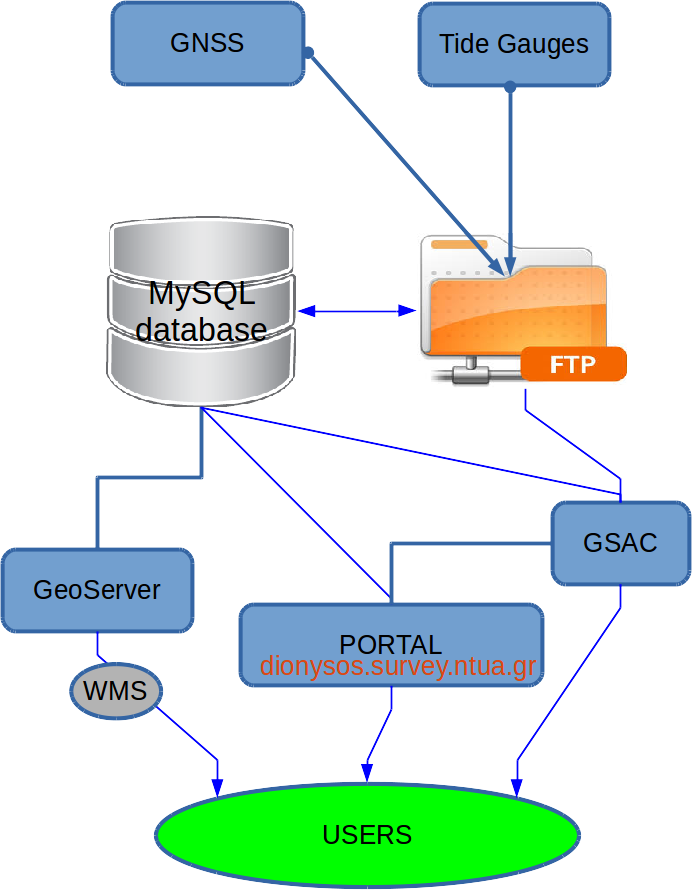
\includegraphics[width=.8\textwidth]{img/flowc.png}
%        \caption{Flowchart of the individual platform modules.}
%        \label{fig:mits}
%        \end{center}
%    \end{figure}
%    \column{.5\textwidth}
%    \begin{figure}
%        \begin{center}
%        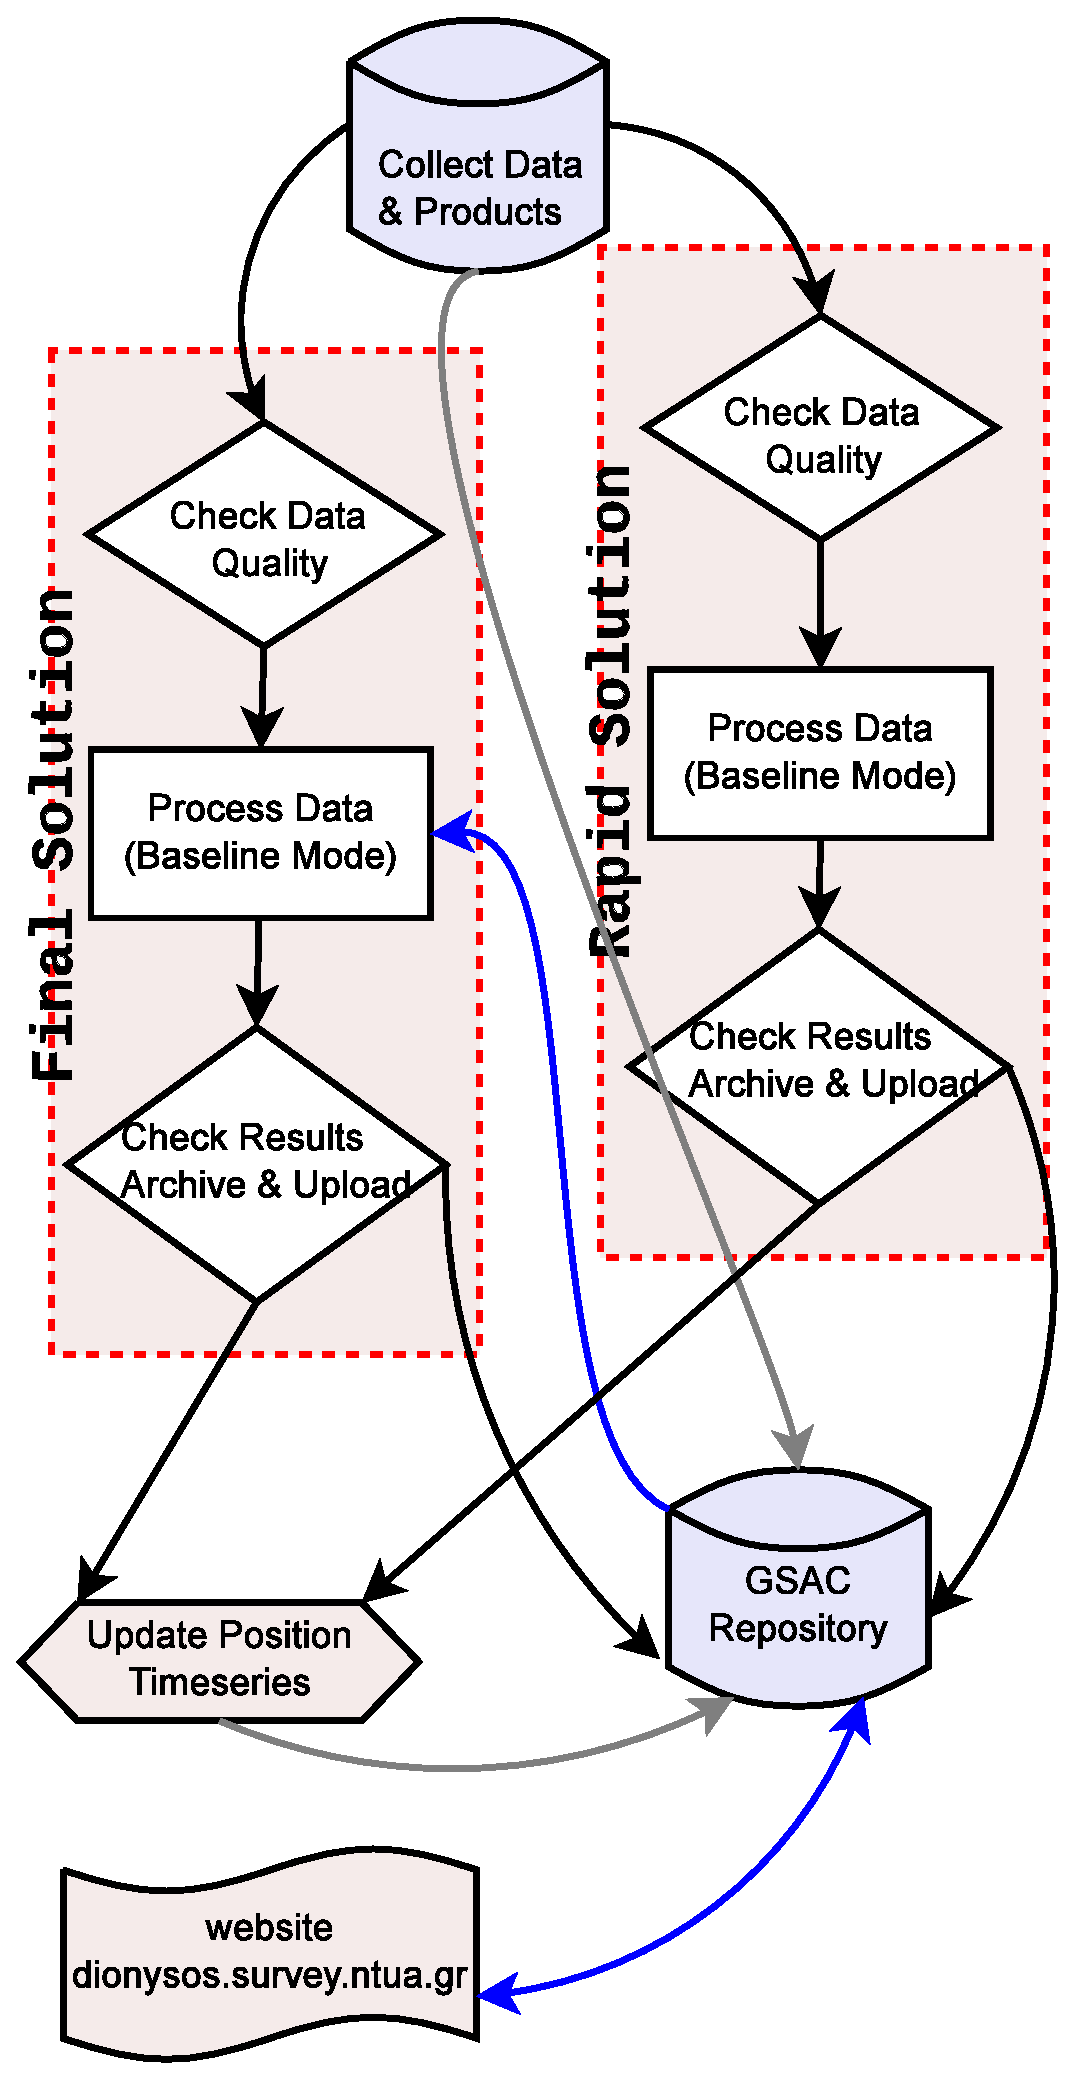
\includegraphics[width=.5\textwidth]{img/Diagram1.eps}
%        \caption{Flowchart of the processing scheme.}
%        \label{fig:dgrm}
%        \end{center}
%    \end{figure}
%  \end{columns}

\end{frame}

\begin{frame}\frametitle{SEISMO Project}\framesubtitle{}
  In the framework of the SEISMO\footnotemark Project, platform has been upgraded,
  to include:

  \begin{itemize}
    \item more GNSS stations, divided into sub-networks,
    \item manipulation, archiving \& dissemination of GNSS data files,
    \item new processing capabilities (e.g. GPS+GLONASS processing),
    \item automatic archiving and publishing of results (via a dedicated web-site),
    \item integration with GSAC (\cite{gsac}) and MySQL databases,
    \item new results and products
  \end{itemize}

  The platform was in practice re-designed \& re-implemented.

  \footnotetext[1]{South Aegean Geodynamic And Tsunami Monitoring Platform}
\end{frame}

\begin{frame}\frametitle{Status}\framesubtitle{}
\end{frame}

\section{Contribution To EUREF}

\begin{frame}\frametitle{Motivation}\framesubtitle{}
  \begin{itemize}
    \item expand \& modernize our research activity,
    \item contribute to the GNSS community,
  \end{itemize}
\end{frame}

\begin{frame}\frametitle{Data}\framesubtitle{}
  Currently we process whatever we can get our hands on \ldots\\
  Problems:
  \begin{itemize}
    \item Inhomogenous dataset (RINEX, raw files, etc).
    \item Various maintainers, different mentalities.
    \item Different aquisition methods/rates.
    \item Hardly any log files.
    \item Wide variety of equipment (not always included in atx files).
  \end{itemize}
\end{frame}

\begin{frame}\frametitle{Data}\framesubtitle{}
  Network installed/maintained by COMET\footnotemark  \& NTUA.
  \begin{itemize}
    \item<pro@1-> established along the Aegean Arc
    \item<pro@1-> homogenous (geodetic type) equipment
    \item<pro@1-> credible time-span (early 2004 - late 2011)
    \item<con@1-> data aquisition stoped at late 2011
    \item<con@1-> equipment is old \& GPS-only
    \item<con@1-> needs repairing
  \end{itemize}
  \footnotetext[1]{Center for Observation and Modeling of Earthquakes, \url{http://comet.nerc.ac.uk/}}
\end{frame}

\begin{frame}\frametitle{Data}\framesubtitle{}
  Network maintained by GEIN/NOA\footnotemark. Sites established by various institutes
  (NTUA, UNAVCO, MIT).
  \begin{itemize}
    \item<pro@1-> covers (sparsely) all of Greece 
    \item<pro@1-> credible time-span (newest stations at 2012)
    \item<con@1-> inconsistent providers (for some stations)
    \item<con@1-> no log files
  \end{itemize}
  \footnotetext[1]{National Observatory of Athens \url{http://www.gein.noa.gr/services/GPS/noa\_gps.html}}
\end{frame}

\begin{frame}\frametitle{Data}\framesubtitle{}
  Network installed/maintained by Tree-Company\footnotemark.
  \begin{itemize}
    \item<pro@1-> dense network, covers all of Greece
    \item<pro@1-> homogenous (geodetic type) equipment
    \item<con@1-> limited time-span (late 2013 onwards)
    \item<con@1-> no log files
    \item<con@1-> comercial usage oriented
  \end{itemize}
  \footnotetext[1]{URANUS network \url{http://www.uranus.gr/}}
\end{frame}

\begin{frame}\frametitle{Data}\framesubtitle{}
  Network installed/maintained by HEPOS\footnotemark (Greek Cadastre Service). 
  \begin{itemize}
    \item<pro@1-> dense network, covers all of Greece
    \item<pro@1-> homogenous (geodetic type) equipment
    \item<con@1-> credible time-span (late 2013 onwards)
    \item<con@1-> limited access ($\sim$5 stations)!!
  \end{itemize}
  \footnotetext[1]{\url{http://www.hepos.gr/}}
\end{frame}

\begin{frame}\frametitle{Data}\framesubtitle{}
  Network installed/maintained by CRLab\footnotemark. 
  \begin{itemize}
    \item<pro@1-> credible time-span
    \item<pro@1-> only covers the Corinth Rift
    \item<con@1-> inconsistent providers
    \item<con@1-> no log files \& equipment changes
  \end{itemize}

  Santorini Network. 
  \begin{itemize}
    \item<con@1-> localized
    \item<con@1-> limited time-span
  \end{itemize}

  \footnotetext[1]{Corinth Rift Laboratory \url{http://webobs.crlab.eu/}}
\end{frame}

\begin{frame}\frametitle{Processing}\framesubtitle{}

\begin{columns}[T] % align columns
\begin{column}{.28\textwidth}
  The core tool/software is Bernese GNSS Software v5.2\cite{bernese}.\\
  \medskip
  Integration with 
  \begin{itemize}
    \item MySQL database,
    \item Python library
    \item GSAC
    \item wrappers (shell)
  \end{itemize}
\end{column}%
\hfill%
\begin{column}{.68\textwidth}
\begin{tikzpicture}[ every annotation/.style = {draw,
                     fill = white, font = \large}]

  \path[mindmap,concept color=black!40,text=white,
    every node/.style={concept,circular drop shadow, scale=.4},
    root/.style = {concept color=black!40,
      font=\normalsize\bfseries,text width=5em},
    level 1 concept/.append style={font=\normalsize\bfseries,
      sibling angle=50,text width=7.7em,
    level distance=20mm,inner sep=0pt},
    level 2 concept/.append style={font=\bfseries,level distance=15mm},
  ]

  node[root] {Bernese GNSS Software v5.2} [clockwise from=0]
    child[concept color=blue!60] {
      node {bernutils Python library} [clockwise from=90]
      child { node[concept] {github repo} }
      child { node[concept] {modules for Bernese output/control files} }
      child { node[concept] {modules for products} }
    }
    child[concept color=blue] {
      node[concept] {MySQL Database} [clockwise from=0]
      child { node[concept] {Bernese .STA} }
      child { node[concept] {IGS log files} }
      child { node[concept] {stations/networks/products} }
    }
    child[concept color=red] {
      node[concept] {/bin wrappers \& utils } [clockwise from=270]
      child { node[concept] {glue everything together} }
      child { node[concept] {various utilities \& formating} }
    }
    child[concept color=yellow!60!black] {
      node[concept] { GSAC } [clockwise from=220]
      child { node[concept] {RINEX} }
      child { node[concept] {products} }
    }
    child[concept color=green!40!black] {
      node[concept] { WebPage } [clockwise from=300]
    }
    \end{tikzpicture}
\end{column}%
\end{columns}
\end{frame}

\begin{frame}\frametitle{Processing}\framesubtitle{}
\end{frame}

\section{Web Resources}

\begin{frame}\frametitle{Web Resources}\framesubtitle{Visit, Browse, Interact, Comment}
\begin{itemize}
    \item \textbf{Dionysos Satellite Observatory} \url{http://dionysos.survey.ntua.gr/}  %%{http://dionysos.survey.ntua.gr/}
    \item \textbf{GSAC repository} \url{http://dionysos.survey.ntua.gr/dsoportal/_datacenter/gsacrepos.html} %%{http://dionysos.survey.ntua.gr/dsoportal/\_datacenter/gsacrepos.html}
    \item \textbf{Ftp site} \url{http://dionysos.survey.ntua.gr/dsoportal/_datacenter/ftpdata.html}  %%{http://dionysos.survey.ntua.gr/dsoportal/\_datacenter/ftpdata.html}
    \item \textbf{Kefallonia earthquake} \url{http://dionysos.survey.ntua.gr/dsoportal/_projects/supersites/cephalonia/}  %%{http://dionysos.survey.ntua.gr/dsoportal/\_projects/supersites/cephalonia/}
    \item \textbf{Ionospheric Remote Sensing} \url{http://dionysos.survey.ntua.gr/dsoportal/_projects/IonoRemSens/}  %%{}
\end{itemize}
\end{frame}

\section{Thank you}
\begin{frame}\frametitle{}\framesubtitle{}
    \begin{center}
    Thank you very much for your attention !
    \end{center}
\end{frame}

\begin{frame}[allowframebreaks]
  \frametitle<presentation>{References}
  \begin{thebibliography}{10}

%  \beamertemplatebookbibitems
%  \bibitem{Autor1990}
%    A.~Autor.
%    \newblock {\em Introduction to Giving Presentations}.
%    \newblock Klein-Verlag, 1990.

  \beamertemplatearticlebibitems

    %% Bernese
    \bibitem{bpe}
    Dach R., Hugentobler U., Fridez P., Meindl M.
    \newblock Bernese GPS Software Version 5.0
    \newblock {\em Astronomical Institute, University of Bern}, 2007.

    %% Papoutsis, Santorini
    \bibitem{papoutsis}
    Papoutsis I., Papanikolaou X., Floyd M., Ji K. H., Kontoes C., Paradissis D., Zacharis V.
    \newblock Mapping inflation at Santorini volcano, Greece, using GPS and InSAR
    \newblock {\em Geophysical Research Letters}, 40(2):267-272, 2013

    %% Sakkas, Kephalonia
    \bibitem{sakkas}
    Sakkas V., Lagios E.
    \newblock Fault modelling of the early-2014 $\sim$ M6 Earthquakes in Cephalonia Island (W. Greece) based on GPS measurements
    \newblock {\em Tectonophysics}, Volumes 644–645,184-196, 2015, Pages 184-196

    %% Diaforoi, sar kephalonia
    \bibitem{sarkefalonia}
    Merryman Boncori J.P., Papoutsis I., Pezzo G., Tolomei C., Atzori S., Ganas A., Karastathis V., Salvi S., Kontoes C., Antonioli A.
    \newblock The February 2014 Cephalonia Earthquake (Greece): 3D Deformation Field and Source Modeling from Multiple SAR Techniques
    \newblock {\em Seismological Research Letters}, Vol.86(1), 2015

    %% Unavco GSAC
    \bibitem{gsac}
    UNAVCO
    \newblock GSAC -- Geodetic Seamless Archive Centers: Open-source Software for Geodesy Data Repositories
    \newblock {\em available at} \url{https://www.unavco.org/software/data-management/gsac/gsac.html}

    %% Unavco IGB08
    \bibitem{igb08}
    P. Rebischung
    \newblock IGb08: an update on IGS08
    \newblock {\em IGSMAIL [6663]} \url{http://igscb.jpl.nasa.gov/pipermail/igsmail/2012/007853.html}, 2012

    %% Unavco vmf1
    \bibitem{vmf1}
    Boehm J., B. Werl, and H. Schuh (2006)
    \newblock Troposphere mapping functions for GPS and very long baseline interferometry from European Centre for
    Medium-Range Weather Forecasts operational analysis data
    \newblock {\em Journal of Geophysical Research}, vol. 111, B02406, 2006

  \end{thebibliography}
\end{frame}

\end{document}
